\chapter{The Klein-Gordon Field}

\nonumsec{Summary}
\begin{itemize}
  \item 整章内容都是基础, 需要掌握所有公式的推导
  \item Peskin \& Schroeder对标量场进行量子化(从书中第20页开始)的方法很奇怪, 可直接参考笔记 \ref{subsubsec: KG_Field_expression} 一节中的方法——①\ 求得标量场运动方程的解; ②\ 利用等时对易关系(此时已经将场看作了算符)计算场展开式中系数(也是算符)的对易关系
  \item 正则量子化定义了单粒子态:
        \begin{equation*}
          |\mathbf{p}\rangle = \sqrt{2E_{\mathbf{p}}}a^{\dagger}_{\mathbf{p}}|0\rangle
        \end{equation*}
  \item Noether守恒荷($j^\mu$为Noether守恒流):
        \begin{equation*}
          Q \equiv \int j^0\ d^3x \quad (\int {\rm in\ all\ space})
        \end{equation*}
  \item 能动量张量:
        \begin{equation*}
          T^{\mu}_{\phantom{\mu}\nu}\equiv \frac{\partial \mathcal{L}}{\partial (\partial_{\mu} \phi)} \partial_{\nu} \phi - \mathcal{L}\delta^{\mu}_{\phantom{\mu}\nu}
        \end{equation*}
  \item 费曼传播子(\textbf{标量场}):
        \begin{equation*}
          \langle 0|T\phi(x)\phi(y)|0 \rangle = D_F(x-y)\equiv \int \frac{d^4 p}{(2\pi)^4} \frac{i}{p^2 - m^2 +i\epsilon} e^{-ip\cdot (x-y)}
        \end{equation*}
\end{itemize}
\pagestyle{general}

\section{The Necessity of the Field Viewpoint}

这里提到需要将场量子化的一个原因是: 由于爱因斯坦关系$E = mc^2$的存在, 任何相对论性过程中都有可能出现正负粒子对, 所以用只对有限个自由度进行了量子化的理论来解释是不够的.
而对于能量较低的情况, 我们可以考虑一个存在时间极短的态, 此时由于不确定性原理$\Delta E \cdot \Delta t = \hbar /2$的存在, 这个态中会产生很多“虚粒子”, 所以\textbf{量子场论}, 或着说可以处理数目不定的自由度的相对论性量子理论是必要的.

同时还有一个原因是关于因果性的.
紧随其后的计算就是经典理论中关于传播振幅$U(t)$的计算, 结果表明它们违背了因果律.

\begin{mybox}{对于场的简单理解}
  \begin{itemize}
    \item 一大堆小弹簧(?)(参考\textit{Goldstein}第13章).
    \item 某种实体在时空中的分布, 它是时空坐标$x^\mu$的函数, 是一个基础的力学量. (更简单更好的理解! )
  \end{itemize}
\end{mybox}
\begin{mybox}{常用的场}
  \begin{itemize}
    \item $\phi(x)$: 标量场(比如希格斯场)
    \item $A_\mu(x)$: 矢量场(电磁场)
    \item $\psi(x)$: 旋量场
  \end{itemize}
\end{mybox}

\subsection{P.14 - Eq-1}

当$E = \mathbf{p}^2/2m$时,
\begin{equation}
  \displaybreak
  \begin{aligned}
    U(t) & = \langle \mathbf{x}|e^{-i(\mathbf{p}^2/2m)t}|\mathbf{x}_0\rangle                                                                                                                         \\
         & = \int d^3p \langle \mathbf{x}| e^{-i(\mathbf{p}^2/2m)t} |\mathbf{p}\rangle \langle \mathbf{p}| \mathbf{x}_0 \rangle                                                                      \\
         & = \int d^3p \ e^{-i(\mathbf{p}^2/2m)t} \langle \mathbf{x}|\mathbf{p}\rangle \langle \mathbf{p}| \mathbf{x}_0\rangle                                                                       \\
         & = \int d^3p \ e^{-i(\mathbf{p}^2/2m)t} \biggl(\frac{1}{2\pi}\biggr)^\frac{3}{2} e^{i\mathbf{p}\cdot\mathbf{x}} \biggl(\frac{1}{2\pi}\biggr)^\frac{3}{2} e^{-i\mathbf{p}\cdot\mathbf{x}_0} \\
         & = \frac{1}{(2\pi)^3} \int d^3p \ e^{-i(\mathbf{p}^2/2m)t} e^{i\mathbf{p}\cdot(\mathbf{x}-\mathbf{x}_0)}                                                                                   \\
         & = \biggl(\frac{m}{2\pi it}\biggr)^\frac{3}{2} e^{im(\mathbf{x}-\mathbf{x}_0)^2/2t} .
  \end{aligned}
\end{equation}

最后一步直接使用高斯积分公式.

\begin{mybox}{一维高斯积分公式}
  \begin{equation}
    \int_{-\infty}^{\infty}dx\ e^{-cx^2}e^{\pm ibx} = \sqrt{\frac{\pi}{c}}e^{-b^2/4c}.
  \end{equation}
\end{mybox}

\subsection{P.14 - Eq-2}

当$E = \sqrt{\mathbf{p}^2+m^2}$时,
\begin{equation}
  \begin{aligned}
    U(t) & = \mathinner{\langle \mathbf{x}|}e^{-it\sqrt{\mathbf{p}^2+m^2}}\mathinner{|\mathbf{x}_0\rangle}                                                                                            \\
         & = \frac{1}{(2\pi)^3} \int d^3p \ e^{-it\sqrt{\mathbf{p}^2+m^2}} e^{i\mathbf{p}\cdot(\mathbf{x}-\mathbf{x}_0)}                                                                              \\
         & = \frac{1}{(2\pi)^3} \int p^2\sin\theta dp d\theta d\varphi \ e^{-it\sqrt{p^2+m^2}} e^{ip|\mathbf{x}-\mathbf{x}_0|\cos\theta}                                                              \\
         & = \frac{1}{(2\pi)^2} \int_0^\infty p^2 dp \ e^{-it\sqrt{p^2+m^2}} \int_0^\pi d\theta \sin\theta \ e^{ip|\mathbf{x}-\mathbf{x}_0|\cos\theta}                                                \\
         & = -\frac{i}{(2\pi)^2|\mathbf{x}-\mathbf{x}_0|} \int_0^\infty dp \ p\ e^{-it\sqrt{p^2+m^2}} \int_0^\pi d(ip|\mathbf{x}-\mathbf{x}_0|\cos\theta) \ e^{ip|\mathbf{x}-\mathbf{x}_0|\cos\theta} \\
         & = -\frac{i}{(2\pi)^2|\mathbf{x}-\mathbf{x}_0|} \int_0^\infty dp \ p\ e^{-it\sqrt{p^2+m^2}} (e^{-ip|\mathbf{x}-\mathbf{x}_0|}-e^{ip|\mathbf{x}-\mathbf{x}_0|})                              \\
         & = \frac{1}{2\pi^2|\mathbf{x}-\mathbf{x}_0|} \int_0^\infty dp \ p\ \sin(p|\mathbf{x}-\mathbf{x}_0|) e^{-it\sqrt{p^2+m^2}}.
  \end{aligned}
\end{equation}

第三行中, 我们把向量$(\mathbf{x}-\mathbf{x}_0)$的方向设为了$z$-axis的正方向.

\subsection{P.15 - Figure 2.1}

两个事件之间的间隔是洛伦兹标量, 即
\begin{equation}
  (x-x_0)^2 = -s^2,
\end{equation}
因为是类空间隔, 所以有个负号.

我们把$x_0$作为原点, 令$x'=x-x_0$, 空间分量只考虑一维($x'=(t',x')$), 则有
\begin{equation}
  x'^2-t'^2=s^2,
\end{equation}
这就是洛伦兹变换下$x'$满足的关系, 即为图中所画的双曲线.

\section{Elements of Classical Field Theory}

注意这里在讨论初末状态时, 直接将时空坐标零分量$x^0$取为了定值.
实际上在不同的空间点, 初末状态的$x^0$可以取不同的值, 只需要保证边界是类空超曲面即可.

\begin{mybox}{个人理解}
  只有边界是类空超曲面时, 向空间的无穷远处积分才能到达时间上的边界.
  可以画个图感受一下.
\end{mybox}

\subsection{P15 - (2.2) (2.3)}

这里的
\begin{equation}
  \frac{\partial \mathcal{L}}{\partial(\partial_\mu \phi)}\delta(\partial_\mu \phi),
\end{equation}
具体可以写成
\begin{equation}
  \frac{\partial \mathcal{L}}{\partial\dot\phi}\delta  \dot{\phi}+\frac{\partial \mathcal{L}}{\partial(\bm{\nabla} \phi)}\delta(\bm{\nabla} \phi),
\end{equation}
这里和下面的计算中出现的都不是四矢量的内积, 而是各分量偏微分的和的简写(可以全部展开算一遍).
于是最后的Euler-Lagrange equation也可以写为
\begin{equation}
  \frac{\partial}{\partial t}\biggl(\frac{\partial \mathcal{L}}{\partial\dot\phi}\biggr) + \bm{\nabla} \biggl(\frac{\partial \mathcal{L}}{\partial(\bm{\nabla} \phi)}\biggr) - \frac{\partial \mathcal{L}}{\partial \phi} = 0,
\end{equation}
这在利用薛定谔场的 Lagrangian 导出薛定谔方程的时候很有用.

而关于这里的边界项$\partial_\mu \bigl(\frac{\partial \mathcal{L}}{\partial(\partial_\mu \phi)}\delta \phi \bigr)$, 注意要分别考虑时间和空间分量(书中也提到了).
\begin{mybox}{薛定谔场的Lagrangian}
  \begin{equation}
    \mathcal{L}_{Schr\ddot{o}dinger} = i\hbar\psi^\dagger\frac{\partial \psi}{\partial t} - \frac{\hbar^2}{2m}\bm{\nabla}\psi^\dagger\bm{\nabla}\psi - V(\mathbf x)\psi^\dagger\psi.
  \end{equation}
\end{mybox}

\subsection{P16 - Hamiltonian Field Theorem}

这里关于哈密顿形式的场论并没有讲完(没有导出运动方程).
导出运动方程要给出场变量和其共轭动量之间的对易/反对易关系, 再计算Heisenberg equation得到运动方程.
\begin{mybox}{Heisenberg equation}
  \begin{equation}
    i\frac{\partial}{\partial t}\mathcal{O} = [\mathcal{O}, H].
  \end{equation}
\end{mybox}


Hamiltonian Field Theorem实际上是和Lagrangian Field Theorem不同的路径.
而为了保证它能给出正确的运动方程, 正则量子化的方法只有两种, 也就是上面提到的(等时)对易/反对易关系.

\subsection{P17 - Noether's Theorem}

我此前的疑惑是: 由书中(2.11)推导, 任意一个对场的全局变换($\alpha$ 为常数)都会导致Lagrangian变化一个4-divergence, 这是不是意味着任意一个对场的全局变换都是对称变换呢?

首先我们考虑书中(2.11)用Euler-Lagrange方程简化表达式的含义.
这一步简化意味着我们只考虑了由最小作用量原理决定的\cemph{物理}的场分布(对应经典力学中由最小作用量原理决定的粒子运动轨道).
根据Weinberg的说法, 此时任意一个对于\cemph{物理}的场分布的全局变换确实都会使书中(2.10)成立, 但\cemph{对称变换}的含义是使得(2.10)成立的对\cemph{任意}场分布的变换, 所以“任意的全局变换都是对称变换”肯定是错误的.

因此我对Noether's theorem的理解是这样的:
\begin{enumerate}
  \item 第一步是检查某变换是否为一个对称变换, 即检查该变换是否保证书中(2.10)成立.
        大多数情况下, 直接将对于某个对场的变换(2.9)代入Lagrangian中即可.

        (\textit{评论})在实际计算时, 大多数我们所关心的对场的变换并不会影响Lagrangian的形式(没有$\mathcal{J}^{\mu}$这一项); 而对于会使Lagrangian变化一个4-divergence的变换, 我们在这一步中既检查了它是否为对称变换, 同时也得到了$\mathcal{J}^{\mu}$的形式.
        例如书中的第二个例子中, 时空平移不仅影响场, 也影响了同为洛伦兹标量Lagrangian本身, 即为上述第二种情况.
  \item 第二步中, 我们在形式上计算Lagrangian的变化, 得到(2.11)式后用Euler-Lagrange方程去掉其第二项.
        这样, 我们得到了考虑了最小作用量原理后的, 由我们对场的变换导致的$\Delta \mathcal{L}(\phi, \partial_\mu \phi)$的形式.
        而由于此项仍需满足书中(2.10), 我们令它等于前面的$\mathcal{J}^{\mu}$后即可得到守恒流.

        (\textit{评论})这一步只是为了得到守恒流关于$\phi, \partial_\mu \phi$的函数表达式.
        可以这样考虑: 如果Lagrangian的形式不变, 则有$\mathcal{L}'-\mathcal{L}=\mathcal{L}-\mathcal{L}=0$ (什么都得不到); 而考虑了最小作用量原理后, $\mathcal{L}'-\mathcal{L}=\mathcal{L}_{(\Delta)}+\mathcal{L}_{(\rm Euler)}-\mathcal{L}=\partial_{\mu}j^{\mu}=0$, $j^{\mu}$即为我们想得到的守恒流表达式.
\end{enumerate}

\begin{mybox}{}
  更好的导出守恒流的方式也许是考虑局域变换, 详见Weinberg书中讲解或Hagen Kleinert课件中 8.1.2 一节.
\end{mybox}

\subsection{P18 - (2.13)}
\begin{equation}
  \begin{aligned}
    \frac{dQ}{dt} & = \int \partial_0 j^0 d^3 x                                      \\
                  & = \int (\partial_\mu j^\mu - \bm{\nabla}\cdot\mathbf{j}) \ d^3 x \\
                  & = - \int \bm{\nabla}\cdot\mathbf{j}\ \ d^3 x                     \\
                  & =0.
  \end{aligned}
\end{equation}

\subsection{P18 - (2.15)}

在求复数场运动方程时, 往往会将场$\phi$和它的共轭$\phi^*$ (共轭转置$\phi^\dagger$) 当作独立的场处理, 但实际上它们之间存在着约束关系.
可以认为是独立的变量的原因如下 (参见\href{https://arxiv.org/abs/1110.5013v5}{这篇笔记}第56页下方):

考虑作用量$S[\phi,\phi^*]$, 其动力学方程由变分原理给出:
\begin{equation*}
  \delta S = \int d^4x\ (A\delta\phi + A^*\delta\phi^*) = 0.
\end{equation*}

\begin{enumerate}
  \item 认为$\phi$与$\phi^*$独立, 则立刻可以写出运动方程:
        \begin{equation*}
          \left\{\begin{array}{c}
            A^{\phantom{*}} = 0 \\
            A^* = 0
          \end{array}\right..
        \end{equation*}

  \item 将$\phi$的两个分量$\phi_r$和$\phi_i$作为独立变量,
        \begin{align*}
          \phi^{\phantom{*}} & = \phi_r + i\phi_i  \\
          \phi^*             & = \phi_r - i\phi_i,
        \end{align*}
        由变分原理得到的结果为
        \begin{equation*}
          \delta S = \int d^4x\ [A(\delta\phi_r+\delta\phi_i) + A^*(\delta\phi_r-\delta\phi_i)] = 0,
        \end{equation*}
        则运动方程:
        \begin{equation*}
          \left\{\begin{array}{c}
            A + A^* = 0 \\
            A - A^* = 0
          \end{array}\right.\Rightarrow A = A^* = 0,
        \end{equation*}
\end{enumerate}
两种方法得到的结果一致.

\section{The Klein-Gordon Field as Harmonic Oscillators}

\subsection{P20 - (2.21) \textasciitilde \ (2.28)} \label{subsubsec: KG_Field_expression}

这里有一种更好的导出标量场表达式的方法.

首先我们把对易关系修改为\textbf{等时对易关系}:
\begin{equation}
  \bigl[\phi(t, \mathbf{x}), \pi(t, \mathbf{y})\bigr] = i\delta^{(3)}(\mathbf{x} - \mathbf{y}),
\end{equation}
而后将$\phi(x)$表达为
\begin{equation}
  \phi(\mathbf{x}, t) = \int \frac{d^3 p}{(2\pi)^3}e^{i\mathbf{p \cdot x}}\phi(\mathbf{p}, t),
\end{equation}
其中的$\phi(\mathbf{p}, t)$为(在上式中同时对两端做积分 $\int e^{-i\mathbf{p'\cdot x}} d^3 x$ )
\begin{equation}
  \phi(\mathbf{p}, t) = \int d^3 x\ e^{-i\mathbf{p \cdot x}}\phi(\mathbf{x}, t),
\end{equation}
由于$\phi^\dagger = \phi$ ($\phi$为实标量场),
\begin{equation}
  \phi^{\dagger}(\mathbf{p}, t) = \int d^3 x\ e^{i\mathbf{p \cdot x}}\phi(\mathbf{x}, t) = \phi(-\mathbf{p}, t).
\end{equation}

接下来考虑运动方程(书中(2.21)), 写出试解:
\begin{equation}
  \phi(\mathbf{p}, t) = a_1(\mathbf{p})e^{-i\omega_p t} + a_2(\mathbf{p})e^{i\omega_p t},
\end{equation}
而
\begin{equation}
  \phi^{\dagger}(\mathbf{p}, t) = a_1^{\dagger}(\mathbf{p})e^{i\omega_p t} + a_2^{\dagger}(\mathbf{p})e^{-i\omega_p t}.
\end{equation}

而$\phi^{\dagger}(\mathbf{p}, t) = \phi(-\mathbf{p}, t)$, 则
\begin{equation}
  \left\{\begin{array}{c} a_1^{\dagger}(\mathbf{p}) = a_2(\mathbf{-p})\\ a_2^{\dagger}(\mathbf{p}) = a_1(\mathbf{-p})\end{array}\right..
\end{equation}

于是$\phi(x)$可以表示为(将$a_1(\mathbf{p})$替换为$\frac{1}{\sqrt{2\omega_\mathbf{p}}} a(\mathbf{p})$):
\begin{equation}
  \begin{aligned}
    \phi(\mathbf{x}, t) & = \int \frac{d^3 p}{(2\pi)^3}e^{i\mathbf{p \cdot x}}\Bigl(a_1(\mathbf{p})e^{-i\omega_p t} + a_2(\mathbf{p})e^{i\omega_p t}\Bigr)                                \\
                        & = \int \frac{d^3 p}{(2\pi)^3}\Bigl(a_1(\mathbf{p})e^{-i\omega_p t +i\mathbf{p \cdot x}} + a_1^{\dagger}(-\mathbf{p})e^{i\omega_p t+i\mathbf{p \cdot x}}\Bigr)   \\
                        & = \int \frac{d^3 p}{(2\pi)^3}\Bigl(a_1(\mathbf{p})e^{-i\omega_p t + i\mathbf{p \cdot x}} + a_1^{\dagger}(\mathbf{p})e^{i\omega_p t - i\mathbf{p \cdot x}}\Bigr) \\
                        & = \int \frac{d^3 p}{(2\pi)^3} \frac{1}{\sqrt{2 \omega_\mathbf{p}}} \Bigl(a(\mathbf{p})e^{-ipx} + a^{\dagger}(\mathbf{p})e^{+ipx}\Bigr).
  \end{aligned}
\end{equation}

值得注意的是, 书中把$a(\mathbf{p})$写为了$a_\mathbf{p}$, 实际上理解为函数就可以了.

\begin{mybox}{个人理解}
  量子化的步骤: 引入正则对易关系, 然后解对应的运动方程.

  例如这里我们首先引入对易关系使得基础力学量$\phi(x),\pi(x)$成为了算符, 然后尝试解K-G方程.
  由于量子化后的方程形式和经典情形下的相同, 我们便可以从经典解出发进行尝试.
  而对于微分方程, 只要能试出正确的解并验证其完备性, 就可以将其作为通解.
\end{mybox}

\subsection{P21 - (2.26)下面那一段}

关于求$a_\mathbf{p}$和$a^{\dagger}_\mathbf{p}$的表达式: 将(2.25)和(2.26)系数凑合适, 加减消去其中一个后, 再同时对两端做积分$\int e^{-i\mathbf{p'\cdot x}} d^3 x$即可.

\begin{mybox}{}
  \begin{center}
    \large \bfseries 确实很easy, Peskin \& Schroeder没有骗你.
  \end{center}
\end{mybox}

\subsection{P22 - (2.33)}

此处计算(以及相关的许多计算)可能要用到如下的关系:
\begin{equation}
  \begin{aligned}
    \int_{-\infty}^{+\infty}\frac{d^3 p}{(2\pi)^3}f(\mathbf p) & = \int_{+\infty}^{-\infty}\frac{d^3 (-p)}{(2\pi)^3}f(-\mathbf p) \\
                                                               & = -\int_{+\infty}^{-\infty}\frac{d^3 p}{(2\pi)^3}f(-\mathbf p)   \\
                                                               & = \int_{-\infty}^{+\infty}\frac{d^3 p}{(2\pi)^3}f(-\mathbf p).
  \end{aligned}
\end{equation}

\subsection{P22 - (2.34)}

建议记这个公式:
\begin{equation}\label{eq: delta_on_function}
  \delta(f(x)) = \sum_i \frac{\delta(x-x_i)}{|f'(x_i)|},
\end{equation}
其中$x_i$是$f(x)$的根.
参考 \href{https://zh.wikipedia.org/wiki/狄拉克δ函数#與函數的復合}{$\delta$函数的维基百科页面}.

\subsection{P23 - (2.40)} \label{subsubsec: Invar_Delta}

我们计算另一个类似的不变积分, $\Delta(x; m)$.

Invariant Delta-Function:
\begin{equation}
  \Delta(x; m) = -i\int\frac{d^3 p}{(2\pi)^3} \frac{1}{2E_\mathbf{p}}(e^{-ipx} - e^{+ipx}).
\end{equation}


$\Delta(x; m)$可写为洛伦兹不变的形式(其中$\varepsilon(x)$为符号函数):
\begin{equation}
  \Delta(x; m) = -i\int \frac{d^4 p}{(2\pi)^4}(2\pi)\varepsilon(p_0) \delta(p^2 - m^2)e^{-ipx},
\end{equation}

\textit{证明}:
\begin{equation}
  \begin{aligned}
    r. h. s. & = -\frac{i}{(2\pi)^3}\int d^3 p \biggl\{ \int_{0}^{\infty}dp^0\delta\Bigl((p^0)^2 - E_\mathbf{p}^2\Bigr)e^{-ipx} - \int_{-\infty}^{0}dp^0\delta\Bigl((p^0)^2 - E_\mathbf{p}^2\Bigr)e^{-ipx} \biggr\} \\
             & = -\frac{i}{(2\pi)^3}\int d^3 p \biggl\{ \int_{0}^{\infty}dp^0\frac{1}{2E_\mathbf{p}}\Bigl[\delta(p^0 - E_\mathbf{p}) + \delta(p^0 + E_\mathbf{p}) \Bigr]e^{-ipx}                                    \\
             & \qquad \qquad \qquad \quad -
    \int_{-\infty}^{0}dp^0\frac{1}{2E_\mathbf{p}}\Bigl[\delta(p^0 - E_\mathbf{p}) + \delta(p^0 + E_\mathbf{p}) \Bigr]e^{-ipx}\biggr\}                                                                               \\
             & = -\frac{i}{(2\pi)^3} \int d^3 p \frac{1}{2E_\mathbf{p}} \Bigl(e^{-iE_\mathbf{p} t + i \mathbf{p} \cdot \mathbf{x}} - e^{+iE_\mathbf{p} t + i \mathbf{p} \cdot \mathbf{x}}\Bigr)                     \\
             & = -\frac{i}{(2\pi)^3} \int d^3 p \frac{1}{2E_\mathbf{p}} \Bigl(e^{-iE_\mathbf{p} t + i \mathbf{p} \cdot \mathbf{x}} - e^{+iE_\mathbf{p} t - i \mathbf{p} \cdot \mathbf{x}}\Bigr)                     \\
             & = \Delta(x; m).
  \end{aligned}
\end{equation}

注意其中$p^2 - m^2 = (p^0)^2 - \mathbf{p}^2 - m^2 = (p^0)^2 - E_\mathbf{p}^2$.

\section{The Klein-Gordon Field in Space-Time}

我们在此笔记的 \ref{subsubsec: KG_Field_expression} 中就已经得到了包含时间的形式, 无须再考虑这一步.

\subsection{P27 - (2.52)}
这里考虑\href{https://zh.wikipedia.org/wiki/柯西积分定理}{柯西积分定理},
沿$L_1, L_2$构成的闭合回路积分值为0.

\begin{figure}[htbp]
  \centering
  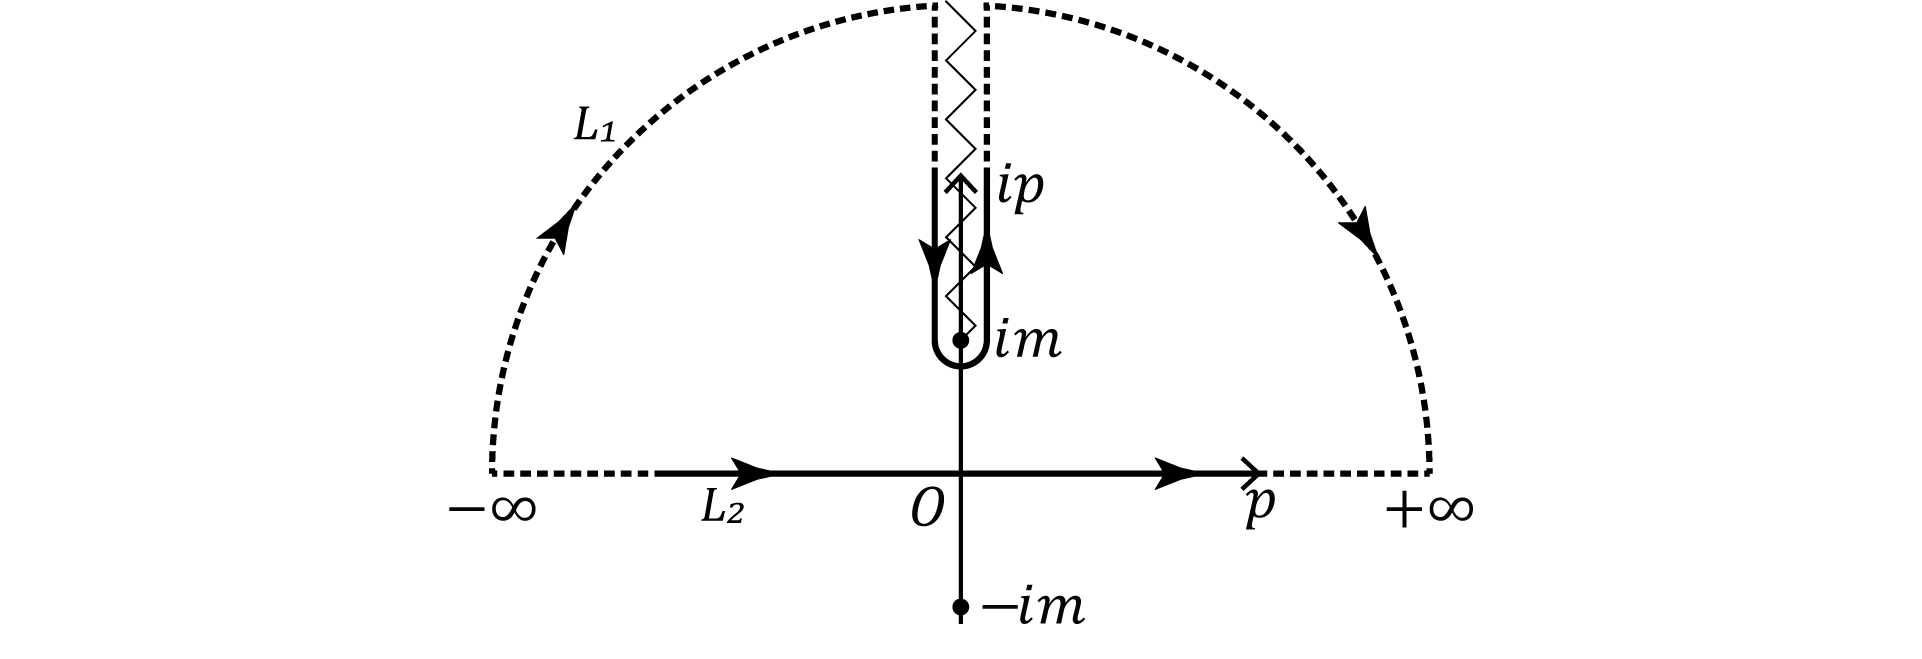
\includegraphics[width = 0.8\textwidth]{P27_2.52.png}
  \caption{Push contour}
  \label{fig: pushcon}
\end{figure}

因此, 若记
\begin{equation}
  f(p) = \frac{pe^{ipr}}{\sqrt{p^2+m^2}},
\end{equation}
并将$p$视为复数, 则有
\begin{equation}\label{eq: push_contour}
  \begin{aligned}
    \int_{L_2}dp\ f(p) & = \int_{L_1}dp\ fp                                  \\
                       & = \int_{\gamma_2}p\ f(p) + \int_{\gamma_1}dp\ f(p),
  \end{aligned}
\end{equation}
其中积分路径为
\begin{equation*}
  \begin{aligned}
    \gamma_1: p(\rho) = i\rho, \rho\in[m,+\infty], \\
    \gamma_2: p(\rho) = i\rho, \rho\in[+\infty,m],
  \end{aligned}
\end{equation*}
这里选择从上半平面积分是因为当$|p|\to\infty$时, $f(p)$在上半平面一致收敛为0.
因此, 两个无穷大$1/4$圆弧上积分值为0; 再考虑到$im$处无穷小半圆弧上的积分值为0, 我们就得到了笔记 \eqref{eq: push_contour} 式的第二行.

点$p = \pm im$是$\sqrt{p^2+m^2}$的支点(branch point).
从分支左侧到右侧时, 需要考虑图 \ref{fig: pushcon} 中所示的分支切割(branch cut), 此时$p^2+m^2$获得了$2\pi$的相位, 即$\sqrt{p^2+m^2}$获得了相位$e^{i\pi}$.
因此,
\begin{equation}
  \begin{aligned}
    \int_{L_2}dp\,f(p) & = \int_{\gamma_2}dp\,f(p) + \int_{\gamma_1}dp\,f(p)                     \\
                       & = \int_{\gamma_2}dp\,\frac{pe^{ipr}}{\sqrt{p^2+m^2}}
    + \int_{\gamma_1}dp\,\frac{pe^{ipr}}{e^{i\pi}\sqrt{p^2+m^2}}                                 \\
                       & = -2\int_{\gamma_1}dp\,\frac{pe^{ipr}}{\sqrt{p^2+m^2}}                  \\
                       & = 2i\int_{m}^{\infty}d\rho\,\frac{\rho e^{-\rho r}}{\sqrt{\rho^2-m^2}},
  \end{aligned}
\end{equation}
将积分结果带回即可得到书中(2.52)式.

\subsection{P28 - (2.53)}

这个commutator用此笔记的 \ref{subsubsec: Invar_Delta} 中的$\Delta$可以表示为:
\begin{equation}
  [\phi(x), \phi(y)] = i\Delta(x-y; m).
\end{equation}

\begin{mybox}{个人理解}
  可以这样解释的原因是: 在量子力学中我们将两个态的内积的模的平方解释为该态可被观测到的概率, 是可观测量.
  而书中前面虽将$\phi(x) |0\rangle$类比为了$|x\rangle$, 但没有赋予其其他含义(可以理解为这个传播振幅无法与可观测量联系起来, 故无法传递信息).
  而算符$\phi(x), \phi(y)$的对易关系与量子力学中算符的对易关系的含义相同.
\end{mybox}

\subsection{P30 - (2.54)}

第二行第二项的$e$指数项中除了把$E_\mathbf{p}$写为了$-(-E_\mathbf{p})$以外, 还做了变换$\mathbf{p} \rightarrow -\mathbf{p}$.

最后一步反着算比较容易: 在最后一行的式子中计算关于$p^0$的积分, 从下方闭合积分路径, 使用留数定理就可以得到第二行的表达式(最后一行表达式中的那个$(-1)$是因为从下方闭合了积分路径); 而这里当$(x_0 - y_0)>0$才从下方闭合积分路径的原因是只有这样$e^{-ip(x - y)}$才在无穷远处为零.

\subsection{P30 - (2.56)}

首先注意:
\begin{equation}
  \partial_\mu \theta(x^0) = g_{0\mu} \delta(x^0) \label{eq: partial_on_delta}.
\end{equation}

第一行: 对阶跃函数求一次导, 再应用分部积分后会得到
\begin{equation}
  \partial_0 \Bigl(\delta(x_0 - y_0)\langle 0|[\phi(x), \phi(y)]|0\rangle \Bigr)-\delta(x_0 - y_0)\partial_0\langle 0|[\phi(x), \phi(y)]|0\rangle,
\end{equation}
其中第一项等于0的原因可以粗略理解为: $x_0 \neq y_0$时, $\delta(x_0 - y_0)$等于0; $x_0 = y_0$时, $\langle 0|[\phi(x), \phi(y)]|0\rangle$等于0.

第二行: 注意使用此笔记的 \eqref{eq: partial_on_delta} 式及书中的(2.47).

第三行: Klein-Gordon equation.

\subsection{P30 - (2.57)}

给等式两边作用微分算符$(\partial^2 + m^2)$, 再比较两边的形式, 就可以得到(2.57)下面的表达式.

\subsection{P31 - (2.59)}

这里极点的计算有个小trick: 我们得到$p^0 = \pm\sqrt{E_\mathbf{p}^2 - i\epsilon}$后, 对小量$\epsilon$展开可得$p^0 = \pm (E_\mathbf{p} - \frac{1}{2}i\epsilon)$, 这时只要令$\epsilon^* = \frac{1}{2}\epsilon$即可(都是同阶无穷小).
